%!TEX encoding = UTF-8 Unicode
%!TEX root = ../paper.tex
\section{Recovery}
\label{sec:recovery}
Tenants initiate a recovery when they detect intrusions. When Shuttle enters recovery mode, it generates a list of requests to replay and asks for the \ac{PaaS} controller to launch a set of \textit{replay instances}. Shuttle may also ask for additional database and application server instances, or they may be launched automatically by the \ac{PaaS} platform when it detects additional load, in case auto-scaling is supported. A non-tampered snapshot, which is previous to the intrusion instant, is selected. The multi-thread HTTP client of each replay instance fetches requests from the \emph{Shuttle Storage} and sends them to the application servers, concurrently whenever possible. After replaying all requests issued before the beginning of the recovery, the manager sets the proxy state to \emph{restraining mode} and commands the replay instances to replay the remaining requests (those issued after recovery began). Then, \emph{restraining mode} is disabled. 
The following sections explain this process in detail.

%%%%%%%%%%%%%%%%%%%%%%%%%%%%%%%%%%%%%%%%%%%%%%%%%%%%%%%%%%%%%%%%%%%%%%%%%%%%%%%%%%%%%%%%%%%%%%%%%%%%%%%%%%%%%%%%%%%%%%%%%%%%%%
\subsection{Intrusion Identification}
\label{sec:recovery:detection}
%how the damage is fixed?
The recovery process starts when an intrusion is detected. \LONG{, but the way in which this is done is out of the scope of the work.} Intrusions may tamper the database \LONG{, e.g., modifying data,} or the application server instances \LONG{, e.g., changing the code of the application}. In order to fix the vulnerabilities that may have lead to intrusions, Shuttle supports the following actions: 1) update the application software; 2) identify a set of tampered database items; 3) add, modify or remove logged requests; 4) launch cleaned database or application server instances.

If tenants update the application software, they have to ensure that the application's interface remains compatible with the requests that will be replayed. If the database is tampered using user requests, the tenant has to identify the malicious user requests. For instance, the tenant can provide the set of suspicious database items to Shuttle and it will resolve the set of requests that accessed the suspicious items after the estimated intrusion moment. Knowing the suspicious requests, the tenants shall use Shuttle to add, modify or remove the past requests to remove accidental or malicious behaves. 

%%%%%%%%%%%%%%%%%%%%%%%%%%%%%%%%%%%%%%%%%%%%%%%%%%%%%%%%%%%%%%%%%%%%%%%%%%%%%%%%%%%%%%%%%%%%%%%%%%%%%%%%%%%%%%%%%%%%%%%%%%%%%
\subsection{Dependency graph}
\label{sec:recovery:dependencies}

%What is it? how it is generated?
A \emph{dependency graph} consists of nodes that represent requests and edges that establish dependencies between them (Figure \ref{fig:selectiveGraph}). Dependencies between requests are established using the following rules: 1) a request $R_A$ is dependent upon request $R_B$ if there is a data item $x$ such that $R_A$ reads $x$ and $R_B$ performs the latest update on $x$; 2) dependencies are transitive except when requests perform blind writes, i.e., requests write items without read them first \cite{itdb}\LONG{cite{Ammann2002}}

Previous solutions for relational databases extract the dependencies using a pre-defined per-transaction type template \cite{itdb} \LONG{cite{Ammann2002}}, or change the relational database management system code to extract read dependencies \cite{phoenix}. In contrast, Shuttle uses the database proxy to log the database accesses. Periodically, each database proxy traverses, in background, the \emph{operation list} of each data item to collect the new accesses and to generate the dependencies between requests. The Shuttle manager processes the dependencies to update the dependency graph. An alternative approach is to pull the dependencies from each database node only before the recovery process and generate the dependency graph when needed. The dependency graph is implemented as a hash table. Keys of the hash table are the \acf{RID}. Each value of the hash table contains the requests that depend on the associated request, i.e., the requests that execute after this one. A scalable implementation can use a distributed hash table or a graph-oriented database.

%false positives: detected but not exist
The above method may lead to \emph{false positives}, i.e., to flag dependencies that do not exist. For instance, a request may read a data item but not use it to compute the written value, so there is no real dependency. Although tracking variables used by each request during its execution might solve this particular case \cite{goel}, it would require modifying the code interpreter (e.g., Zend Engine for PHP), which would constrain Shuttle to a set of specific languages. As our approach uses the dependencies to group the requests that can be executed concurrently, false dependencies imply a performance penalty but do not cause data loss or inconsistent state.

%false negatives: not detected but exist
Complex queries on a relational database may lead to \emph{false negatives}, for instance when a read operation would have been executed on a deleted data item if this data item had not been deleted before the request execution \cite{Xie2008}. In contrast with SQL queries that access the data items that match a query, the \ac{CRUD} interface of most key-value stores specifies, in a deterministic and apriori manner, the data item that will be accessed. Shuttle logs every access, even when the data items do not exist, keeping the \emph{operation list} of the deleted data items to track further operations.


%%%%%%%%%%%%%%%%%%%%%%%%%%%%%%%%%%%%%%%%%%%%%%%%%%%%%%%%%%%%%%%%%%%%%%%%%%%%%%%%%%%%%%%%%%%%%%%%%%%%%%%%%%%%%%%%%%%%%%%%%%%%%%
\subsection{Replay}
\label{sec:recovery:replay}

Shuttle aims to support a large range of applications in which the user requests access a distributed database without using transactions. This assumption contrasts with previous recovery systems that collect the order requests based on the semantics of the application they consider (e.g., \cite{undoForOperators}) or leverage the serialization provided by snapshot isolation to do it (e.g., \cite{goel}). Moreover, requests executed concurrently during  normal execution, may  depend on each other, e.g., the first reads an item written by the second and the second reads an item written by the first.

%how I sort the requests?
We propose a new approach to order the requests for replaying that consists on sorting the requests per \emph{start-end order}, instead of using a dependency graph. Requests are replayed ordered by their start instant. Moreover, if a request starts before the end of another request, then they were executed concurrently and they are also re-executed concurrently. 
%DB Ordering
Yet, re-execution of concurrent requests is not deterministic, e.g., due to multi-thread servers, messaging systems, etc. Therefore our novel approach uses the \emph{operation list} to make parallel replay deterministic, by forcing operations to a data item during replay to follow the order established by its operation list (Figure \ref{fig:inconsistency_db_order}).

%locked requests
Modifications to the application code or to the sequence of requests may cause the application not to access the same sequence of data items or read/write the same content during the replay phase (Figure \ref{fig:inconsistency_unlock}). If an operation contained in the operation list is not performed, the following operations to the data item are blocked. To address this problem, at the end of each request execution, the \textit{database client interceptor} fetches the list of data items accessed by the request on its first execution and compares them against the ones accessed during the replay process. The database client library invokes the \emph{database proxy} with the keys that have not been accessed to unlock the remaining requests. 


\begin{figure*}[!thp]
  \centering
  \mbox{
          \subfloat[][Ordered by operation list \label{fig:inconsistency_db_order}]{
              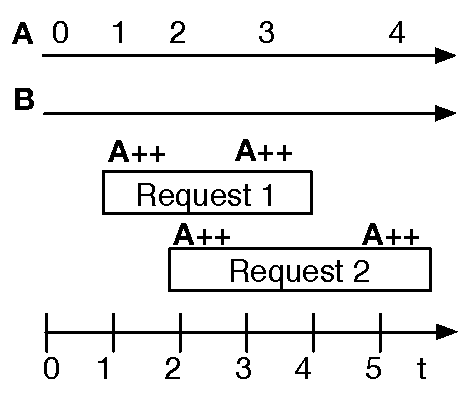
\includegraphics[width=0.20\linewidth]{images/inconsistency_db_order}
          }

          \subfloat[][Operation unlock \label{fig:inconsistency_unlock}]{
              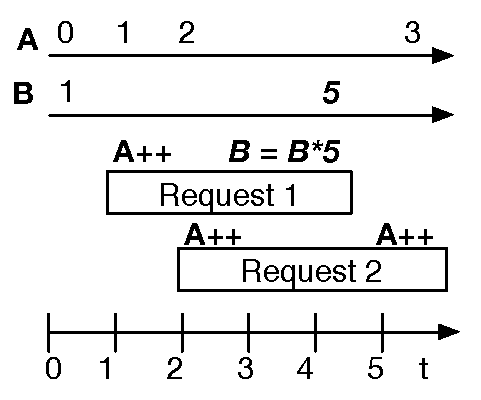
\includegraphics[width=0.20\linewidth]{images/inconsistency_unlock}
          }

          \subfloat[][Consecutive requests \label{fig:inconsistency_serial}]{
              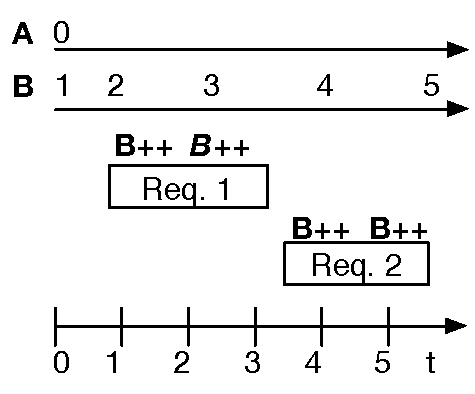
\includegraphics[width=0.20\linewidth]{images/inconsistency_serial}
          }

          \subfloat[][Conflict \label{fig:inconsistency_conflict}]{
              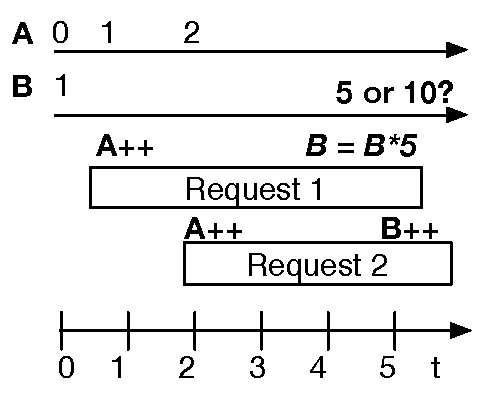
\includegraphics[width=0.20\linewidth]{images/inconsistency_conflict}
          }
  }
  \caption{Replay two requests with different re-execution}
  \label{fig:inconsistency}
  \vspace{-5mm}
\end{figure*}

During replay there may be non-deterministic situations, whenever an access is not contained in the operation list. Consider the case of Figure \ref{fig:inconsistency}. Figure \ref{fig:inconsistency_db_order} represents the first execution of two requests. During the recovery period, the intrusion was removed hence requests access different data items than in the first execution. If the \emph{req.~2} started after the end of \emph{req.~1}, the replay would consistent with the first execution (Figure \ref{fig:inconsistency_serial}). An approach using only the dependency graph would have inconsistent results because the new dependency happens at recovery time.


%Conflict 
The problematic scenario is that the two requests were executed concurrently during their first execution: the \emph{start-end order} defines that \emph{req.~1} and \emph{req.~2} are replayed concurrently (Figure \ref{fig:inconsistency_conflict}). The access to $A$ remains consistent with the first execution (\emph{req.~2} after \emph{req.~1}), since the accesses are constrained by the \emph{operation list} of $A$. However, the final value of $B$ is unpredictable because \emph{req.~1} may write $B$ before or after \emph{req.~2}. Since both requests did not access the data item $B$ during their execution, the operation list does not establish an access order. Therefore, the \emph{req.~1} and \emph{req.~2} may execute in a arbitrary order. The order of these requests is as deterministic as if during the first execution: the operation of \emph{req.~1} can execute before, between or after \emph{req.~2}.

%versioning e conciliamento
In order to turn the replay process more consistent with the first execution, we leverage semantic reconciliation, as in Dynamo \cite{Decandia2007}. The case represented in Figure \ref{fig:inconsistency_conflict} is equivalent to a concurrent update, where two parallel writes are performed on distinct database instances. Each request writes a distinct version resulting in conflicting versions of an item. Developers use the application-assisted conflict resolution interface to merge the versions. In this case, the following read operation would access the values written by the latest operation. In Figure \ref{fig:inconsistency_conflict}, \emph{req.~2} could choose between $5$ and $1$.

%other sources of non-determinism - nao devia estar fora daqui?!
The application shall be deterministic. An application is said to be deterministic if two subsequent executions with the same initial state and user inputs can be guaranteed to have the same final state and outputs. Five of the main sources of non-determinism are: shared memory, thread concurrency, random number generation, timestamps, and message exchanging. We assume requests to be independent thus they do not share memory, and that concurrent threads are independent. The API provided by Shuttle provides deterministic random number generation and timestamps using the \acf{RID} as timestamp and pseudo-random number seed, so the replay of a request will use the same random numbers and timestamp (we consider a single timestamp per request to be enough for most applications). This mechanism is language independent. User requests and database accesses are ordered in a deterministic way using the operation list.


\subsection{Clustering}
\label{sec:recovery:clusters}
%Must execute some requests in parallel
Our preliminary experiments have shown that replaying requests concurrently can reduce the recovery period. We want recovery to take a fraction of the time elapsed since the snapshot from which recovery starts (e.g., if the snapshot was taken a week before, we want recovery to take much less than that period). 

We address this problem grouping the requests into \emph{clusters}. A cluster is a set of requests that have dependencies between them but not from/to requests in other clusters. Clusters are created when the recovery is about to start by inspecting the dependency graph. Since clusters are independent, they execute concurrently by different \emph{replay instance} without synchronization. Requests within the same cluster, are performed in start-end order (Section \ref{sec:recovery:replay}). Given that more requests are executed concurrently, Shuttle launches more application servers and database instances to process the replayed requests. Therefore, the replay phase throughput is bigger than during first execution and the recovery time is minimized. This mechanism is applicable if the graph dependencies remain unchanged during the recovery phase, i.e,. all replayed operations are contained in the operation list but not all operations in the list must be replayed.


%%%%%%%%%%%%%%%%%%%%%%%%%%%%%%%%%%%%%%%%%%%%%%%%%%%%%%%%%%%%%%%%%%%%%%%%%%%%%%%%%%%%%%%%%%%%%%%%%%%%%%%%%%%%%%%%%%%%%%%%%%%%
\subsection{Full and Selective Replay}
\label{sec:recovery:selective_replay}

We propose two approaches for intrusion recovery: full replay and selective replay. Full replay consists in replaying every request done after the  snapshot. Executing many requests takes considerable time, so this approach is adequate for issues detected reasonably fast after they happen, e.g., a few days or weeks. Selective replay re-executes only part of the requests so it is faster than full-replay. However, it requires tenants to provide a set of malicious actions (i.e., requests) $A_{intrusion}$. This set is used to deduce the set of tainted requests $A_{tainted}$. A request is said to be tainted if it is one of the attacker’s requests or if it reads objects written by tainted request \cite{taser,itdb,phoenix}.  The selective replay process is as follows (full replay is simpler so we skip it):

\textbf{1)}\textit{Determine the malicious requests $A_{intrusion}$.}
  Based on initial data such as user session compromised or data items accessed, the tenant determines the requests $A_{intrusion}$ used by the attacker to compromise the application. For instance, $A_{intrusion} = \{R.4\} $ (Figure \ref{fig:selectiveGraph}).
  
\textbf{2)} \textit{Use $A_{intrusion}$ to determine the set of tainted requests $A_{tainted}$.}
  For each request in $A_{intrusion}$, traverse the dependency graph in causality order and add these nodes to $A_{tainted}$ (in the figure $A_{tainted} = \{R.5,R.6,R.7,R.8\}$).

\textbf{3)}\textit{Get the requests needed to obtain the values read by $A_{tainted}$ and their effects.} 
  Instead of storing the input and output of every action or versions of every data item, we propose to replay the actions which $A_{tainted}$ depends on. The data item value is known at the snapshot instant so the algorithm transverses the graph in inverse causality order from each request in $A_{tainted}$ and stores the requests in $A_{replay}$ ($A_{replay} = \{R.2\} \cup A_{tainted}$). $A_{replay}$ is expanded by traversing the graph from each of its elements on causality order to determine the requests which can be affected by the re-execution of $A_{replay}$ ($A_{replay} = A_{replay} \cup R.3$). Requests subsequent to the first snapshot after the latest malicious request may not be repeated if all their read operations read the value contained in the snapshot (version read by $R.8$ is stored in snapshot B).

\textbf{4)}\textit{Determine the replay order.} 
  The set $A_{replay}$ is sorted on non-clustered \emph{start-end order}.

\textbf{5)}\textit{Load the previous data item versions}
  Shuttle loads the version, which is previous to the selected snapshot, of the data items read by the requests in $A_{replay}$.

\textbf{6)} \textit{Replay the requests}
  Requests in $A_{replay}$ are replayed. If an access is not contained in operation list, then a new dependency is established and the requests that accessed the data item during the first execution are also replayed as in \emph{taint propagation via replay} \cite{retro}. For instance, $R.9$ is replayed if it reads an item written during recovery process but not during normal execution. 

\begin{figure}
  \centering
  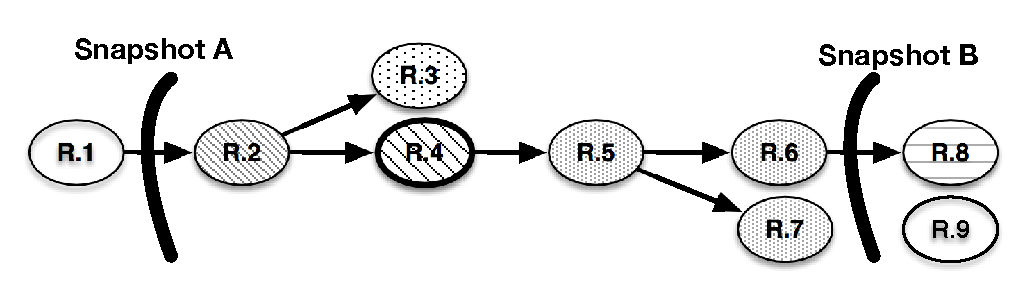
\includegraphics[width=\linewidth]{images/selectiveDependency}
  \caption{{Dependency graph:} $R.1$ is previous to a snapshot $A$; $R.3$ is dependent on $R.2$, which is replayed to get the read values; $R.4$ is a malicious request; $R.5,R.6,R.7$ are tainted; $R.8$ may not be replayed; $R.9$ is independent of the rest.}
  \label{fig:selectiveGraph}
\end{figure}


%----------------------------------------------------------------------------------------------------------------------------
\subsection{Consistency}
\label{sec:recovery:consistency}

An important aspect of a recovery system like Shuttle is the application consistency seen by users. For instance, if a user does an action based on data written by a malicious action, which result of the user action replay is consistent? Since users have a non-deterministic behavior, they may have to be notified if a recovery took place and their data was modified.

Shuttle does not execute requests that returned an error in the first execution. Similarly to other works in the area \cite{undoForOperators}, we assume that these cases are compensated by the user when they happen. As only requests that did not return an error are replayed, Shuttle considers an inconsistency when a request returns an error or a response is different during replay. Shuttle provides the following API for the application programmer to define how inconsistencies are dealt with (Shuttle calls these functions in case they are launched by the tenant):
\begin{enumerate}
  \item \textit{preRecover():} invoked before the beginning of the recovery process.
  \item \textit{handleInconstency(request, previous response, new response, previous keys, new keys, action):} invoked when there is an inconsistency.
  \item \textit{postRecover(statistics, old version, new version):} invoked after the end of the recovery process.
\end{enumerate}

The first function allows tenants to perform a set of actions before the beginning of the recovery process, such as notifying the operations team or taking a new snapshot. 
The second function takes as input the operation that caused the inconsistency as well as the response and keys accessed during the normal execution and during the recovery process. It also takes as argument the action to take. Currently we consider three possible actions: 1) ignore the inconsistency; 2) notify the user of the inconsistency; 3) execute another request. 
Using the \textit{postRecover} function, the tenant has access not only to the statistics of the recovery process but also to an interface to compare the database values before and after the recovery process and the application responses, before exposing the data to the users. 

Besides its users, an application may also interact with external services. We simplify the problem by considering that applications only obtain inputs from external services, disregarding the issue of outputs. The problem is treated in \cite{aire,undoForOperators}. 



%%%%%%%%%%%%%%%%%%%%%%%%%%%%%%%%%%%%%%%%%%%%%%%%%%%%%%%%%%%%%%%%%%%%%%%%%%%%%%%%%%%%%%%%%%%%%%%%%%%%%%%%%%%%%%%%%%%%%%%%%%%%%%
\subsection{Instance Rejuvenation}
\label{sec:recovery:instance_rejuventaion}
% Why? Because the instances can be corrupted
Attackers may exploit system vulnerabilities to tamper application server or database instances, affecting the application integrity or availability. Shuttle interacts with the \ac{PaaS} controller to rejuvenate instances when they are compromised. This process terminates the instances and launches new ones. The PaaS controller initializes the new instances with updated machine images and deploys an updated version of the application code, which may include updates to fix discovered flaws or prevent future intrusions.

We assume new instances to be intrusion-free as the image can be updated to fix previous flaws and their persistent state is renewed. Instances can be launched in a remote site to recover from catastrophic disasters \cite{cloud-disaster}. Tenants are responsible for ensuring that request dependencies remain correct and the updated version API is compatible, or for providing a script to update each request to the new API. Moreover, the selected snapshot has to be consistent according to the updated version specification or every request executed since the application's begin shall be replayed.

This process can be used in a proactive manner to renew instances to remove unknown intrusions \LONG{cite{Castro2002}}\cite{Sousa2010} or to test new application versions to compare its results against the previous version, using the branching mechanism (Section \ref{sec:recovery:runtime_recovery}).


%%%%%%%%%%%%%%%%%%%%%%%%%%%%%%%%%%%%%%%%%%%%%%%%%%%%%%%%%%%%%%%%%%%%%%%%%%%%%%%%%%%%%%%%%%%%%%%%%%%%%%%%%%%%%%%%%%%%%%%%%%%%%%
\subsection{Recovery in Runtime}
\label{sec:recovery:runtime_recovery}
%why?
Shuttle is capable of doing recovery on runtime, i.e., without making the application unavailable for a period of time. To do so, each recovery process is considered to be a new branch, a model inspired in versioning systems such as \emph{git} \cite{git}. A \emph{branch} is a sequence of snapshots (akin to the commits in git). Figure \ref{fig:branches} presents an example with 3 branches and 5 snapshots.

\begin{SCfigure}
  \centering
  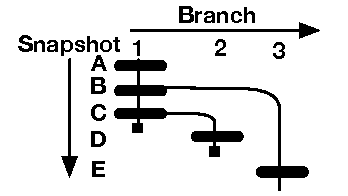
\includegraphics[width=40mm]{images/branches}
  \caption{\footnotesize{Tree model:} 3 branches and 5 snapshots: branch 1 contains snapshots A,B,C;\newline Branch 2 contains D;\newline Branch 3 contains E.}
  \label{fig:branches}
\end{SCfigure}

Each recovery process creates a new branch forking a previous snapshot chosen by the tenant, either explicitly or implicitly (by indicating the initial intrusion instant, selecting implicitly the preceding snapshot). Incoming user requests access only the data of the previous branch keeping the application available, while replayed requests access the created branch without compromising the availability of the application. In addiction, tenants can use the branching mechanism to test their intrusion recovery procedures in background, i.e, without exposing users to test issues.

%branch-path
Since tenants can select previous snapshots, we define a branch as a sequence of non-tampered snapshot, named \emph{branch path}. For instance, the snapshots $E, B, A$ compose the branch 3 (Figure \ref{fig:branches}). Every database instance knows the \emph{branch path} of the previous branch and the newly created branch in use by the requests being replayed.

%How it works? 
Since a novel data item version is created only when the data item is written for the first time during each snapshot, the data item may not have a version for each snapshot (Section \ref{sec:architecture:snapshot}). Therefore, the version to accessed by an operation is defined using the branch path and the \emph{version list} of the data item: operations read the latest version present in the \emph{version list} and in the \emph{branch path} and write the latest version in the branch path. A new version is added to the version list on the first key access to each data item during the replay. This mechanism allows mapping the request to the correct version. Since the \emph{version list} keeps a pointer to the latest version and this reference is updated, the complexity of getting the correct version is $O(1)$. 

%Working explanation
At recovery time, the manager sends the new \emph{branch path} to every database instance. The new incoming users access the, perhaps corrupted, old branch while the requests being replace access the new branch. Therefore, the application remains online, perhaps with a degraded behavior, without exposing downtime to users.

At some point, when the recovery is finishing, the user requests have to start being issued to the new branch. To do so, after replaying the requests, the proxy flag \emph{restraining} is set and every new request is marked with the \emph{restrain} flag. Database accesses marked with \emph{restrain} are delayed. After replaying the requests retrieved during the recovery process, the proxy sets the new branch in the subfield \emph{branch} of \ac{SRD} of the new requests, the \emph{restrain} flag is disabled and the database nodes are notified to proceed the accesses. This mechanism delays the processing of some requests, but this has typically a duration of seconds, compared with a recovery process that may take many minutes or even hours.